\section{Análise do programa fonte}

\begin{frame}[fragile]{Análise e síntese}

    \begin{itemize}
        \item A compilação é composta por duas partes: análise e síntese
        \pause

        \item A análise divide o programa fonte em partes constituintes e as organiza em uma representação intermediária
        \pause

        \item Em geral, a representação intermediária consiste em uma árvore sintática, onde cada nó representa uma operação e cada filho representa um
            operando
        \pause

        \item A síntese constrói o programa alvo a partir desta representação intermediária
    \end{itemize}

\end{frame}

\begin{frame}[fragile]{Exemplo de árvore sintática}

    \begin{figure}
        \centering

        \begin{tikzpicture}
            \node (A) at (0, 4) { $\mathrm{imc}$ };
            \node (B) at (2, 6) { \texttt{=} };
            \node (C) at (4, 4) { \texttt{÷} };
            \node (D) at (2, 2) { $m$ };
            \node (E) at (6, 2) { \texttt{×} };
            \node (F) at (4, 0) { $h$ };
            \node (G) at (8, 0) { $h$ };

            \draw[very thick] (A) to (B);
            \draw[very thick] (C) to (B);
            \draw[very thick] (C) to (D);
            \draw[very thick] (E) to (C);
            \draw[very thick] (E) to (F);
            \draw[very thick] (E) to (G);
        \end{tikzpicture}

        \caption{Árvore sintática da fórmula $\mathrm{imc} = m/h^2$.}
    \end{figure}

\end{frame}

\begin{frame}[fragile]{Análise do programa fonte}

    A análise é composta por três fases:
    \pause

    \begin{enumerate}
        \item \textit{análise linear}: o fluxo de caracteres que compõem o programa alvo é lido, da esquerda para direita, e agrupado em \textit{tokens} (sequência
            de caracteres com significado coletivo)
        \pause

        \item \textit{análise hierárquica}: os \textit{tokens} são ordenados hierarquicamente em coleções aninhadas com significado coletivo
        \pause

        \item \textit{análise semântica}: verificação que garante que os componentes do programa se combinam de forma significativa
    \end{enumerate}

\end{frame}

\begin{frame}[fragile]{Análise léxica}

    Em um compilador, a análise linear também é denominada análise léxica ou esquadrinhamento.
    \pause
    Por exemplo, no enunciado
        \begin{center}
        \code{cpp}{F = 1.8 * C + 32}
        \end{center}
    a análise léxica identificaria os seguintes \textit{tokens}:
    \pause
    \vspace{0.1in}

    \begin{enumerate}
        \item o identificador \code{cpp}{F}
        \pause
        \item o símbolo de atribuição \code{cpp}{=}
        \pause
        \item a constante em ponto flutuante \code{cpp}{1.8}
        \pause
        \item o símbolo de multiplicação \code{cpp}{*}
        \pause
        \item o identificador \code{cpp}{C}
        \pause
        \item o símbolo de adição \code{cpp}{+}
        \pause
        \item a constante inteira \code{cpp}{32}
    \end{enumerate}
\end{frame}

\begin{frame}[fragile]{Análise sintática}

    A análise hierárquica também é denominada análise sintática ou gramatical. Ela agrupa os \textit{tokens} hierarquicamente, em geral em uma
    árvore gramatical.\pause

    \vspace{0.1in}
    A estrutura hierárquica pode ser definida por meio de regras recursivas. \pause Por exemplo, considere as seguintes regras:
    \pause
    \vspace{0.1in}

    \begin{enumerate}
        \item qualquer identificador é uma expressão
        \pause

        \item qualquer número é uma expressão
        \pause

        \item se $E_1$ e $E_2$ são expressões, também são expressões $E_1 + E_2$ e $E_1 * E_2$
        \pause
    
        \item se $I$ é um identificador e $E$ uma expressão, então $I = E$ é um enunciado
    \end{enumerate}

\end{frame}

\begin{frame}[fragile]{Exemplo de árvore gramatical}

    \begin{figure}
        \centering

        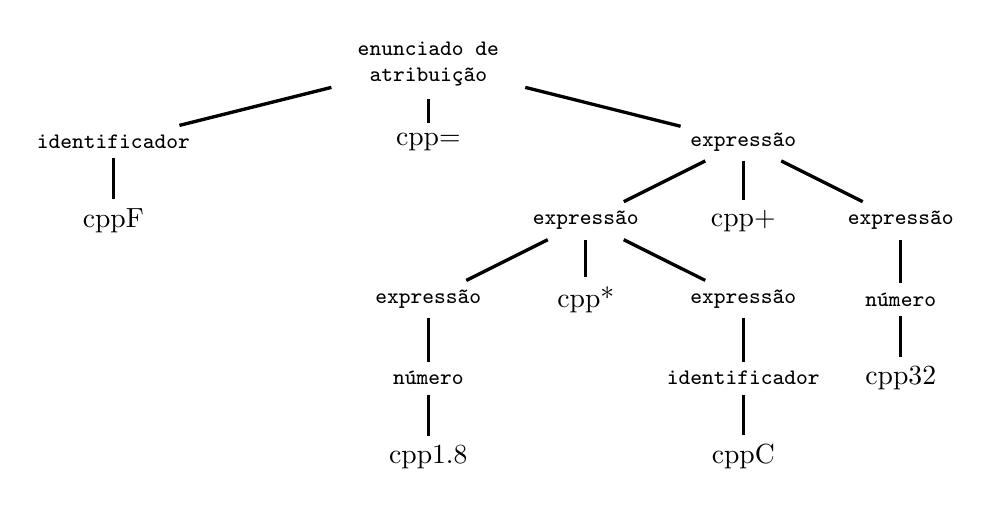
\begin{tikzpicture}
            \node (A) at (0, 5) { \footnotesize \texttt{identificador} };
            \node (A1) at (0, 4) { \code{cpp}{F} };
            \node (B) at (4, 6) { \footnotesize \begin{tabular}{c}\texttt{enunciado de}\\ \texttt{atribuição}\end{tabular} };
            \node (B1) at (4, 5) { \code{cpp}{=} };
            \node (C) at (8, 5) { \footnotesize \texttt{expressão} };
            \node (C1) at (8, 4) { \code{cpp}{+} };
            \node (D) at (6, 4) { \footnotesize \texttt{expressão} };
            \node (D1) at (6, 3) { \code{cpp}{*} };
            \node (E) at (10, 4) { \footnotesize \texttt{expressão} };
            \node (E1) at (10, 3) { \footnotesize \texttt{número} };
            \node (E2) at (10, 2) { \code{cpp}{32} };
            \node (F) at (4, 3) { \footnotesize \texttt{expressão} };
            \node (F1) at (4, 2) { \footnotesize \texttt{número} };
            \node (F2) at (4, 1) { \code{cpp}{1.8} };
            \node (G) at (8, 3) { \footnotesize \texttt{expressão} };
            \node (G1) at (8, 2) { \footnotesize \texttt{identificador} };
            \node (G2) at (8, 1) { \code{cpp}{C} };

            \draw[very thick] (A) to (B);
            \draw[very thick] (A) to (A1);
            \draw[very thick] (B) to (B1);
            \draw[very thick] (C) to (C1);
            \draw[very thick] (D) to (D1);
            \draw[very thick] (E) to (E1);
            \draw[very thick] (E1) to (E2);
            \draw[very thick] (F) to (F1);
            \draw[very thick] (F1) to (F2);
            \draw[very thick] (G) to (G1);
            \draw[very thick] (G1) to (G2);
            \draw[very thick] (C) to (B);
            \draw[very thick] (C) to (D);
            \draw[very thick] (E) to (C);
            \draw[very thick] (D) to (F);
            \draw[very thick] (D) to (G);
        \end{tikzpicture}

        \caption{Árvore gramatical do enunciado \code{cpp}{F = 1.8 * C + 32}}
    \end{figure}

\end{frame}

\begin{frame}[fragile]{Análise semântica}

    \begin{itemize}
        \item A análise semântica verifica potenciais erros semânticos no programa alvo
        \pause

        \item Ela usa a árvore da análise sintática para identificar operadores e operandos das expressões e enunicados
        \pause

        \item Ela também faz a verificação de tipos
        \pause

        \item Caso os tipos dos operandos não sejam compatíveis com os tipos esperados pelos operadores, esta análise ou retorna um erro ou adicionar uma
        promoção (ou conversão) de tipo, a depender da linguagem alvo
        \pause

        \item Por exemplo, na expressão à direita do enunciado \code{cpp}{F = 1.8 * C + 32}, o operando à esquerda da soma tem tipo ponto flutuante e o da direita
            tipo inteiro: o valor \code{cpp}{32} deve ser promovido para ponto flutuante ou deve ser sinalizado um erro de tipo
    \end{itemize}

\end{frame}

